\documentclass{beamer}
\usepackage[utf8]{inputenc}

\usetheme{Madrid}
\usecolortheme{default}
\usepackage{amsmath}
\usepackage{amssymb,amsfonts,amsthm}
\usepackage{txfonts}
\usepackage{tkz-euclide}
\usepackage{listings}
\usepackage{adjustbox}
\usepackage{array}
\usepackage{tabularx}
\usepackage{gvv}
\usepackage{lmodern}
\usepackage{circuitikz}
\usepackage{tikz}
\usepackage{graphicx}

\setbeamertemplate{page number in head/foot}[totalframenumber]

\usepackage{tcolorbox}
\tcbuselibrary{minted,breakable,xparse,skins}



\definecolor{bg}{gray}{0.95}
\DeclareTCBListing{mintedbox}{O{}m!O{}}{%
  breakable=true,
  listing engine=minted,
  listing only,
  minted language=#2,
  minted style=default,
  minted options={%
    linenos,
    gobble=0,
    breaklines=true,
    breakafter=,,
    fontsize=\small,
    numbersep=8pt,
    #1},
  boxsep=0pt,
  left skip=0pt,
  right skip=0pt,
  left=25pt,
  right=0pt,
  top=3pt,
  bottom=3pt,
  arc=5pt,
  leftrule=0pt,
  rightrule=0pt,
  bottomrule=2pt,
  toprule=2pt,
  colback=bg,
  colframe=orange!70,
  enhanced,
  overlay={%
    \begin{tcbclipinterior}
    \fill[orange!20!white] (frame.south west) rectangle ([xshift=20pt]frame.north west);
    \end{tcbclipinterior}},
  #3,
}
\lstset{
    language=C,
    basicstyle=\ttfamily\small,
    keywordstyle=\color{blue},
    stringstyle=\color{orange},
    commentstyle=\color{green!60!black},
    numbers=left,
    numberstyle=\tiny\color{gray},
    breaklines=true,
    showstringspaces=false,
}
\title{2.8.6}
\date{31st August, 2025}
\author{Vishwambhar - EE25BTECH11025}

\begin{document}

\frame{\titlepage}
\begin{frame}{Question}
Assuming that the straight lines work as the plane mirror for a point, find the image of the point $\brak{1,2}$ in the line $x-3y+4=0$.
\end{frame}

\begin{frame}{Translation}
Translating the system by $\vec{A}=\myvec{4\\0}$ so that the line passes through origin:
\begin{align}
    L=\myvec{1&-3}\myvec{x\\y}=-4;
    \vec{P}=\myvec{1\\2}\\
    \vec{P}_{trans}=\vec{P}-\vec{A}=\myvec{1\\2}-\myvec{-4\\0}=\myvec{5\\2}\\
    L_{trans}=\myvec{1&-3}\myvec{x\\y}=0
\end{align}
\end{frame}

\begin{frame}{Normal Vector}
Finding the normal vector:
\begin{align}
    \vec{N}=\myvec{1&-3}
\end{align}

Finding the unit normal vector:
\begin{align}
    ||\vec{N}||=\sqrt{1^2+\brak{-3}^2}=\sqrt{10}\\
    \vec{n}=\frac{\vec{N}}{||\vec{N}||}=\frac{1}{\sqrt{10}}\myvec{1\\-3}
\end{align}
\end{frame}

\begin{frame}{Reflection Matrix}
Calculating the reflection matrix $R$ is given by the formula $R=I-2\vec{n}\vec{n}^T$
\begin{align}
    R=\myvec{1&0\\0&1}-2\brak{\frac{1}{\sqrt{10}}\myvec{1\\-3}}\brak{\frac{1}{\sqrt{10}}\myvec{1&-3}}
    =\myvec{\frac{4}{5}&\frac{3}{5}\\ \frac{3}{5}&\frac{-4}{5}}
\end{align}


Reflecting the given point:
\begin{align}
    \vec{P'}_{trans}=R.P_{trans}=\myvec{\frac{26}{5}\\ \frac{7}{5}}
\end{align}
\end{frame}

\begin{frame}{Conclusion}
Inverting the translation:
\begin{align}
    \vec{P'}=\vec{P'}_{trans}+\vec{A}=\myvec{\frac{6}{5}\\ \frac{7}{5}}
\end{align}

Thus the final image of the given point is $\vec{P'}=\myvec{\frac{6}{5}\\ \frac{7}{5}}$
\end{frame}

\begin{frame}[fragile]
    \frametitle{C Code}
    \begin{lstlisting}
// reflect.c
#include <math.h>

typedef struct { double x, y; } Point;
typedef struct { double a, b, c; } Line;

/* Stored values for the question */
static Point stored_point = {1.0, 2.0};
static Line  stored_line  = {1.0, -3.0, 4.0};

/* Accessors */
void get_point(double* x, double* y){ if(x)*x=stored_point.x; if(y)*y=stored_point.y; }
void get_line(double* a,double* b,double* c){ if(a)*a=stored_line.a; if(b)*b=stored_line.b; if(c)*c=stored_line.c; }
    \end{lstlisting}
\end{frame}

\begin{frame}[fragile]
    \frametitle{C Code}
    \begin{lstlisting}
/* General reflection across ax+by+c=0 */
void reflect_point_across_line(double x0, double y0,
                               double a, double b, double c,
                               double* xr, double* yr)
{
    double denom = a*a + b*b;
    double t = (a*x0 + b*y0 + c) / denom;
    if(xr) *xr = x0 - 2*a*t;
    if(yr) *yr = y0 - 2*b*t;
}

/* Convenience for stored values */
void reflect_stored(double* xr, double* yr){
    reflect_point_across_line(stored_point.x, stored_point.y,
                              stored_line.a, stored_line.b, stored_line.c,
                              xr, yr);
}
    \end{lstlisting}
\end{frame}

\begin{frame}[fragile]
    \frametitle{Python Code 1}
    \begin{lstlisting}
# solve_reflection.py
import ctypes
from ctypes import c_double, byref

lib = ctypes.CDLL('./problem.so')  # adjust path if needed

# Signatures
lib.reflect_stored.argtypes = [ctypes.POINTER(c_double), ctypes.POINTER(c_double)]
lib.reflect_stored.restype  = None
lib.get_point.argtypes = [ctypes.POINTER(c_double), ctypes.POINTER(c_double)]
lib.get_point.restype  = None
lib.get_line.argtypes  = [ctypes.POINTER(c_double), ctypes.POINTER(c_double), ctypes.POINTER(c_double)]
lib.get_line.restype   = None
    \end{lstlisting}
\end{frame}

\begin{frame}[fragile]
    \frametitle{Python Code 1}
    \begin{lstlisting}
# Read stored inputs
x0 = c_double(); y0 = c_double()
a  = c_double(); b  = c_double(); c  = c_double()
lib.get_point(byref(x0), byref(y0))
lib.get_line(byref(a), byref(b), byref(c))

# Compute reflection
xr = c_double(); yr = c_double()
lib.reflect_stored(byref(xr), byref(yr))

print(f"Point P: ({x0.value}, {y0.value})")
print(f"Line: {a.value}*x + {b.value}*y + {c.value} = 0")
print(f"Reflected image: ({xr.value}, {yr.value})")  # (-1.0, 2.0)
    \end{lstlisting}
\end{frame}

\begin{frame}[fragile]
    \frametitle{Python Code 2}
    \begin{lstlisting}
import sys
sys.path.insert(0, '/home/ganachari-vishwmabhar/Downloads/codes/CoordGeo')
import numpy as np
import matplotlib.pyplot as plt

from line.funcs import *
from triangle.funcs import *

# Given line: x - 3y + 4 = 0  => a=1, b=-3, c=4
a, b, c = 1, -3, 4

P = np.array([1, 2])

x1, y1 = P
den = a**2 + b**2
    \end{lstlisting}
\end{frame}

\begin{frame}[fragile]
    \frametitle{Python Code 2}
    \begin{lstlisting}
x_img = ((b**2 - a**2)*x1 - 2*a*b*y1 - 2*a*c)/den
y_img = ((a**2 - b**2)*y1 - 2*a*b*x1 - 2*b*c)/den
P_img = np.array([x_img, y_img])
# Plot line
x_vals = np.linspace(-5, 5, 100)
y_vals = (-(a*x_vals + c))/b
plt.plot(x_vals, y_vals, 'k-', label='Mirror Line')

# Plot original point and image
plt.scatter([P[0], P_img[0]], [P[1], P_img[1]], c=['r','b'])
plt.text(P[0], P[1], 'P(1,2)', fontsize=12)
plt.text(P_img[0], P_img[1], "P'", fontsize=12)

    \end{lstlisting}
\end{frame}

\begin{frame}[fragile]
    \frametitle{Python Code 2}
    \begin{lstlisting}
# Connect them with perpendicular
plt.plot([P[0], P_img[0]], [P[1], P_img[1]], 'g--', label='Perpendicular')

# Settings
plt.axis('equal')
plt.grid(True)
plt.legend()
plt.title("Reflection of Point (1,2) in Line x - 3y + 4 = 0")
plt.savefig("../figs/plot.png")
plt.show()
    \end{lstlisting}
\end{frame}

\begin{frame}{Plot}
    \begin{figure}
        \centering
        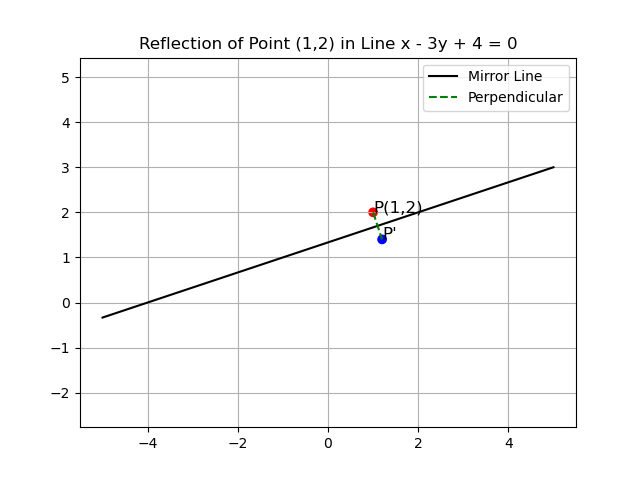
\includegraphics[width=0.5\columnwidth]{../figs/plot.png}
        \caption{Plot of orthogonal vectors $\vec{a}$ and $\vec{b}$.}
        \label{fig:fig}
    \end{figure}
\end{frame}




\end{document}